\documentclass[a4paper,10pt]{article}
\usepackage[a4paper, total={167mm, 245mm}]{geometry}

\usepackage[colorlinks,linkcolor=blue,bookmarks,bookmarksopen,pdfauthor=krom]{hyperref}

\usepackage{fontspec}
\setmainfont[BoldFont={fonts/epkgobld.ttf}]{epkaisho.ttf}

\graphicspath{{images/}}

\usepackage[normalem]{ulem}
\renewcommand{\ULthickness}{0.08em}

\usepackage[compact]{titlesec}
\titlespacing{\section}{0em}{*0}{*0}
\titleformat{\section}{\normalfont\huge}{\thesection}{0em}{}

\setlength\parindent{1em}
\setlength\parskip{0em}
\renewcommand{\baselinestretch}{1.4}

\usepackage{fancyhdr}
\pagestyle{fancy}
\fancyhf{}
\renewcommand\headrulewidth{0pt}

\usepackage{tikz}
\tikzset{>=stealth} % Define Standard Arrow Tip
\definecolor{fontgreen}{RGB}{86, 158, 56}
\definecolor{fontpink}{RGB}{255, 128, 128}
\definecolor{fontyellow}{RGB}{255, 255, 128}
\definecolor{arrowblue}{RGB}{0, 146, 255}

\begin{document}

\fancyfoot[R]{\thepage}

\begin{flushright}
2016/3/26 Revision
\end{flushright}

\vspace{17.5em}

\LARGE
\textbf{\hskip 5em \,OpenToonz}\par
\textbf{\hskip 5em \,Startup Manual}\par
\textbf{\hskip 5em \,Introduction}

\noindent \begin{picture}(0,0)
\put(0,24){
\includegraphics[width=5em]{OpenToonzLogo}}
\end{picture}

\newpage

\phantomsection
\section*{\uline{\hskip -3em \hskip 3em □ Installation Procedure \hskip 8em}}
\addcontentsline{toc}{section}{□ Installation Procedure}

\large

\noindent ① Start the installer

\noindent \begin{picture}(0,0)
\put(72,-90){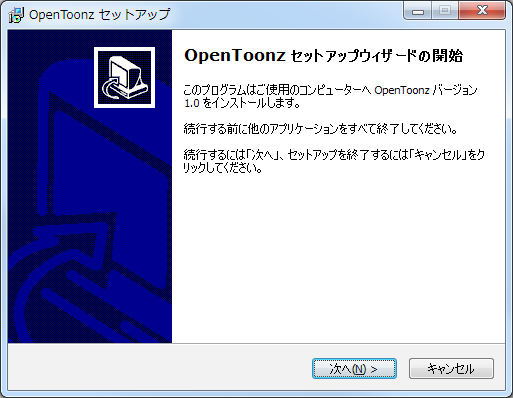
\includegraphics[width=11.5em]{InstallationProcedure1A}}
\put(257,-90){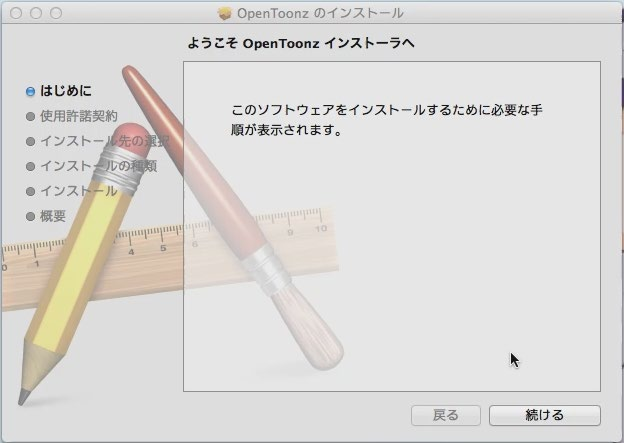
\includegraphics[width=12.5em]{InstallationProcedure1B}}
\end{picture}\\[5.5em]

\noindent ② Read the Terms \& Conditions, if you want to proceed, press the "Agree" button.

\noindent \begin{picture}(0,0)
\put(72,-90){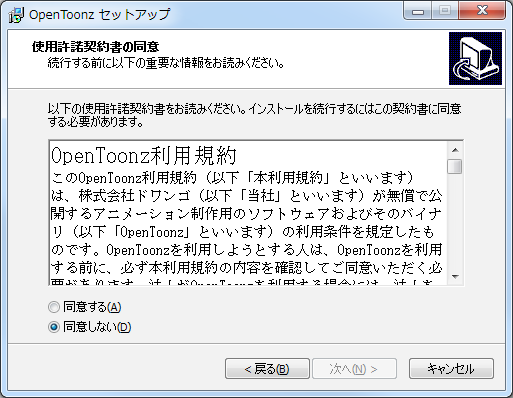
\includegraphics[width=11.5em]{InstallationProcedure2A}}
\put(257,-90){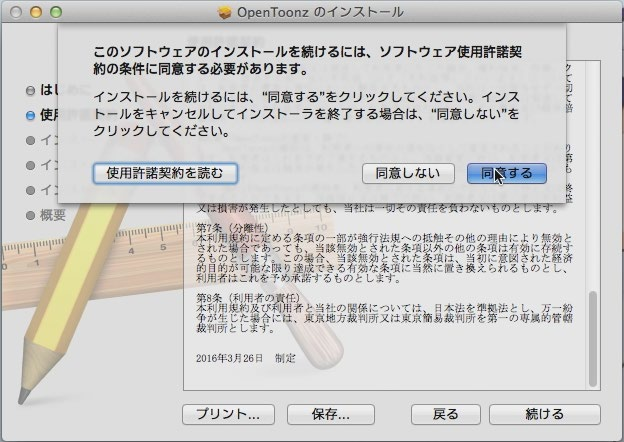
\includegraphics[width=12.5em]{InstallationProcedure2B}}
\end{picture}\\[5.5em]

\noindent ③ Specify the OpenToonz software installation destination

\noindent \begin{picture}(0,0)
\put(72,-90){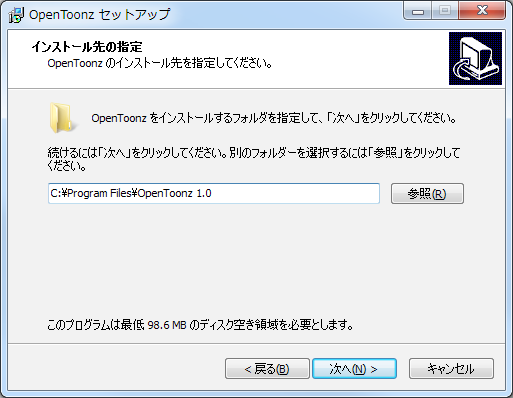
\includegraphics[width=11.5em]{InstallationProcedure3A}}
\put(257,-90){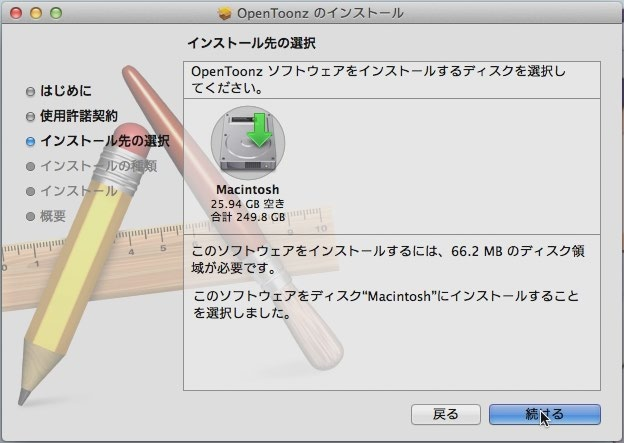
\includegraphics[width=12.5em]{InstallationProcedure3B}}
\end{picture}\\[7.5em]

\noindent ④ (Windows only) Specify the Stuff destination folder.\\[0.5em]
\normalsize
In the case of OS X, Stuff folder location will be pre-determined.\\
You can change the location of this folder (described later on).\\
Also in the case of Windows, the Start menu and desktop icons\\
will be added automatically.

\large

\noindent \begin{picture}(0,0)
\put(329,-20){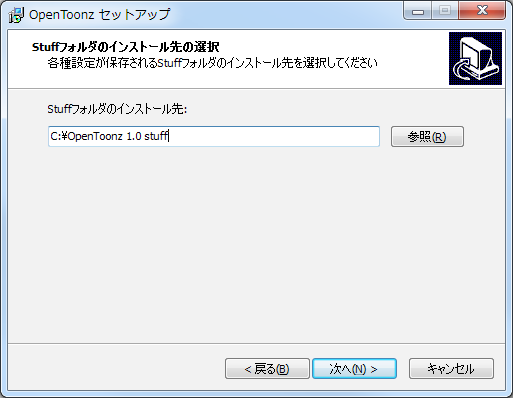
\includegraphics[width=11.5em]{InstallationProcedure4}}
\end{picture}\\[-0.5em]

\noindent ⑤ Once the files have been copied, the installation is complete.

\noindent \begin{picture}(0,0)
\put(72,-98){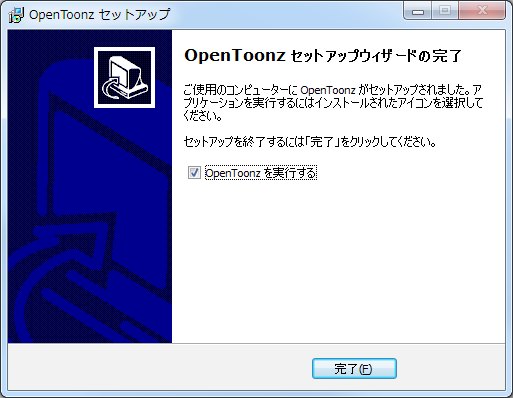
\includegraphics[width=11.5em]{InstallationProcedure5A}}
\put(257,-98){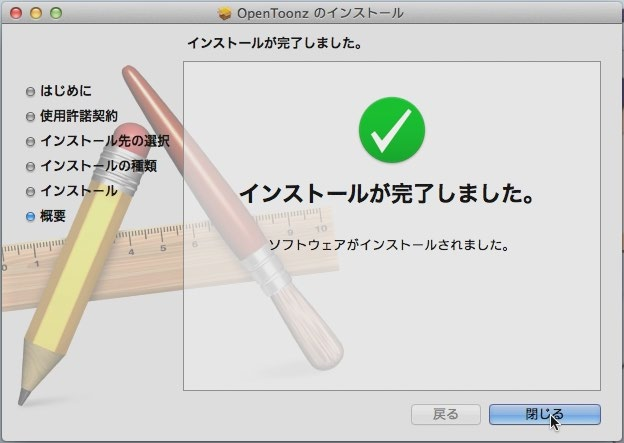
\includegraphics[width=12.5em]{InstallationProcedure5B}}
\end{picture}

\fancyfoot[R]{\thepage
\begin{picture}(0,0)
\put(-523,-50){
\includegraphics[width=58em]{OpenToonzFooter}}
\end{picture}
}

\newpage

\phantomsection
\section*{\uline{\hskip -3em \hskip 3em □ Stuff Folder Information\hskip 7.5em}}
\addcontentsline{toc}{section}{□ Stuff Folder Information}

\normalsize
\noindent The Stuff folder houses various settings of OpenToonz. If more than one user is working on the\\
 same project, creating a shared Stuff folder in the data directory, can unify project settings\\
and work from a common color sample data set.\\
Inside the Stuff folder, there are several additional sub-folders as follows:\\
- cache: Image cache data is temporarily stored here\\
- config: Contains the style sheet, various configuration files, such as the translation file\\
- fxs: This is where the effect preset parameters are saved\\
- library: Pre-prepared material such as video content or audio samples imorted into OpenToonz\\
- profiles: Work environment settings, etc. will be saved here for each user\\
- projects: Project configuration files are saved here\\
- studiopalette: Global color swatch palette, shared by the entire project will be saved here\\
These folders can be moved in the following way even after installation.\\[0.4em]
\par
\large
\noindent ● To change the path of the Stuff folder, etc. (Windows) \normalsize \colorbox{fontpink}{\color{black}Advanced Level}\\
※ With administrator privileges do the following.\\
① Press the Windows key + R, type "regedit" in the "Run" dialog, \& then run it.\\
② The Registry Editor will now open.\\
③ In HKEY\_LOCAL\_MACHINE$\backslash$SOFTWARE$\backslash$OpenToonz$\backslash$OpenToonz$\backslash$1.0, the path to each folder is stored,\\
rewrite the one you want to change using the following key:\par
\ \ \ \ \ "TOONZROOT" \ \ \ \ \ : Stuff folder\par
\ \ \ \ \ "TOONZPROJECTS" \ : projects\par
\ \ \ \ \ "TOONZCACHEROOT" : cache\par
\ \ \ \ \ "TOONZCONFIG" \ \ \ : config\par
\ \ \ \ \ "TOONZPROFILES" \ : profiles\par
\ \ \ \ \ "TOONZFXPRESETS"  : fxs\par
\ \ \ \ \ "TOONZLIBRARY" \ \ : library\par
\ \ \ \ \ "TOONZSTUDIOPALETTE" : studiopalette\\[0.4em]
\par
\large
\noindent ● To change the path of the Stuff folder, etc. (OS X) \normalsize \colorbox{fontpink}{\color{black}Advanced Level}\\
In the case of OS X, the Stuff folder has been saved to /Applications/OpenToonz/OpenToonz\_1.0\_stuff/\\
as the default location after the installation.\\
① From the context menu of the OpenToonz 1.0.app, select "Show Package Contents".\\
② Open SystemVar.ini from Contents/Resources in a text editor.\\
③ As in the above case of Windows, edit the value corresponding to each folder, \& then Save.\\[0.4em]
\par
\large
\noindent ● Other sub-folders inside Stuff folder\\
\normalsize
- doc: Contains Help files of some of the effects that are mounted in OpenToonz\\
- plugins: Copy the plug-in effects files (.plugin) to this folder\\
- sandbox: Contains the set of sandbox projects that are provided by default

\newpage

\phantomsection
\section*{\uline{\hskip -3em \hskip 3em □ OpenToonz Data Handling\hskip 8em}}
\addcontentsline{toc}{section}{□ OpenToonz Data Handling}

\normalsize
\noindent OpenToonz proprietary data formats \& their relationships, are shown in the figure below.

\large
\noindent \begin{picture}(0,0)
\bfseries
\put(60,-240){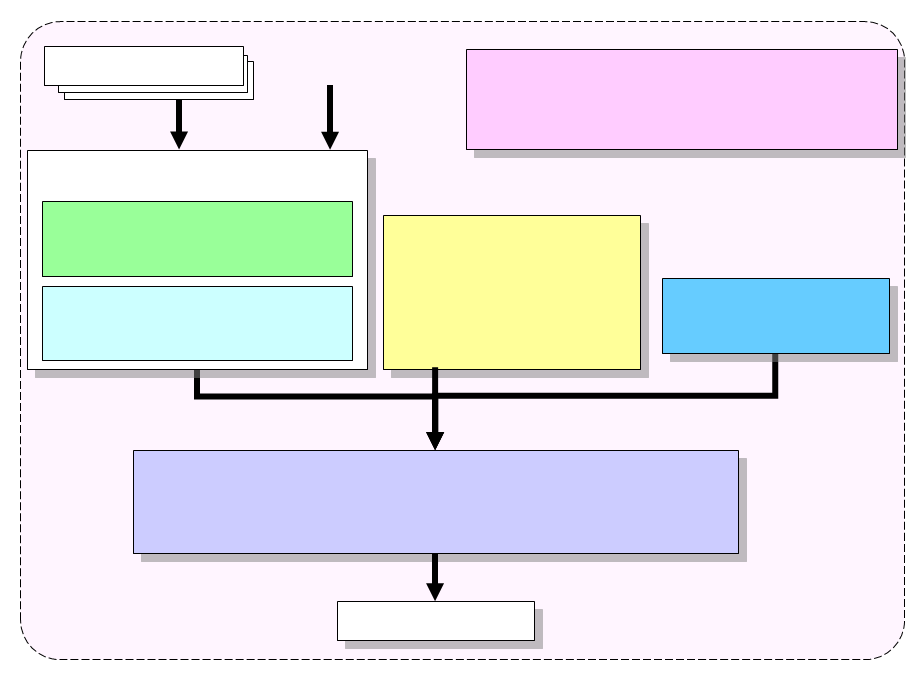
\includegraphics[width=28.5em]{OpenToonzData}}
\put(78,-17){\small Sequence Images}
\put(161,-20){\scriptsize Digital Animation}
\put(237,-20){\small Project File (XML): All Work}
\put(252,-30){\small ・Path of the Working Folder}
\put(252,-40){\small ・Default Values for Settings}
\put(90,-39){\scriptsize Trace}
\put(93,-59){\small Each Cell (Raster)}
\put(77,-75){\small Level File (TLV)}
\put(91,-87){\small ・Raster Image Data}
\put(77,-107){\small Palette File (TPL)}
\put(91,-119){\small ・Palette Data}
\put(205,-81){\footnotesize Each Cell (Vector)}
\put(205,-97){\footnotesize Vector Level File}
\put(205,-107){\footnotesize (PLI)}
\put(205,-117){\footnotesize ・Image + Palette Data}
\put(310,-104){\small General\,Image File}
\put(310,-116){\small (Background,\,etc.)}
\put(151,-150){\scriptsize Place In Time Sheet}
\put(113,-169){\small Scene File (TNZ): Each Cut}
\put(127,-180){\footnotesize ・Path to All of the Material}
\put(247,-180){\footnotesize ・Effects Data}
\put(127,-191){\footnotesize ・Geometric Transform Data}
\put(247,-191){\footnotesize ・Output Settings}
\put(172,-208){\scriptsize Rendering}
\put(188,-224){\small Output\,(Pic/Vid)}
\end{picture}\\[-0.5em]

\noindent \hskip 1em 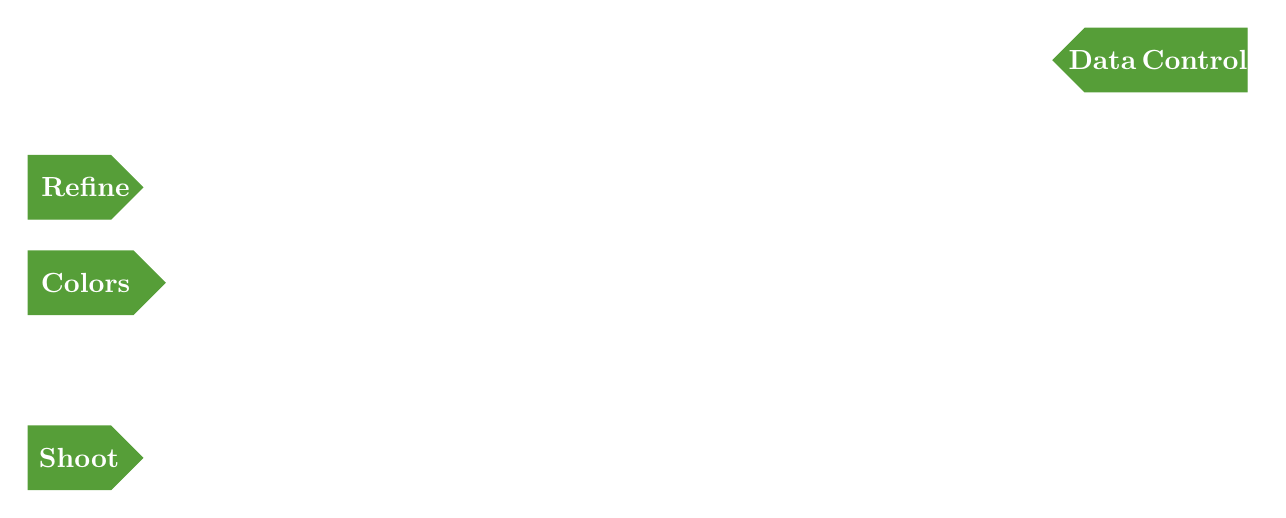
\begin{tikzpicture}
\bfseries
\draw[fill=fontgreen,fontgreen]  (33.2em,0em) --  (32.2em,-1em) --  (33.2em,-2em) -- (38.3em,-2em) -- (38.3em,0em) -- cycle;
\node at (35.5em,-1em) {\textcolor{white}{Data\,Control}};
\draw[fill=fontgreen,fontgreen]  (2.6em,-4em) --  (3.6em,-5em) --  (2.6em,-6em) -- (0em,-6em) -- (0em,-4em) -- cycle;
\node at (1.8em,-5em) {\textcolor{white}{Refine}};
\draw[fill=fontgreen,fontgreen]  (3.3em,-7em) --  (4.3em,-8em) --  (3.3em,-9em) -- (0em,-9em) -- (0em,-7em) -- cycle;
\node at (1.8em,-8em) {\textcolor{white}{Colors}};
\draw[fill=fontgreen,fontgreen]  (2.6em,-12.5em) --  (3.6em,-13.5em) --  (2.6em,-14.5em) -- (0em,-14.5em) -- (0em,-12.5em) -- cycle;
\node at (1.6em,-13.5em) {\textcolor{white}{Shoot}};
\end{tikzpicture}\\[3em]

\noindent ① Toonz Raster Level File\\
\normalsize
The data of the Raster Image Cell. Each file contains 1 of the Image Cell data Frames.\\
The extension is .tlv. (It is referenced by Toonz \& OpenToonz as a Level cell in English.)\\[0.8em]
\large
② Palette File\\
\normalsize
Describes the data of the Pallet from the Cell. The extension is .tpl. As it is written in text, \\
you can see the contents in a text editor such as Notepad.\\[0.2em]
\uline{★ 1 per Cell, there is a paired TLV file with the same name as the TPL file.}\\[0.8em]
\large
③ Toonz Vector Level File\\
\normalsize
The data of the drawn Vector Cell. Each file contains 1 of the Image Cell data Frames,\\
it also contains the Palette data in the same file. The extension is .pli.\\[0.8em]
\large
④ Scene File\\
\normalsize
Describes text data of each Cut. File paths \& material (Toonz Level, Background Image, etc.),\\
Effects data, geometric transforms, \& entries such as output settings. The extension is .tnz.\\[0.8em]
\large
⑤ Project File\\
\normalsize
The path location of all work data (Project Folder), \& describes the default value of the scene\\
 settings. It is written in the form of an XML script.\\[2em]
Roughly speaking,  refine Image data \& Color Palette file (TPL), to complete the Level file (TLV),\\
combine the data of each Cell \& the background material, to complete Scene file (TNZ), it is then\\
 ready for the final shooting process.

\newpage

\phantomsection
\section*{\uline{\hskip -3em \hskip 3em □ OpenToonz Interface\hskip 10em}}
\addcontentsline{toc}{section}{□ OpenToonz Interface}

\normalsize
\noindent OpenToonz interface contains a variety of "panels" that have been prepared for each function.\\
Users can use a combination of these panels freely in the workspace (Room).

\large
\noindent \begin{picture}(0,0)
\put(4,-137){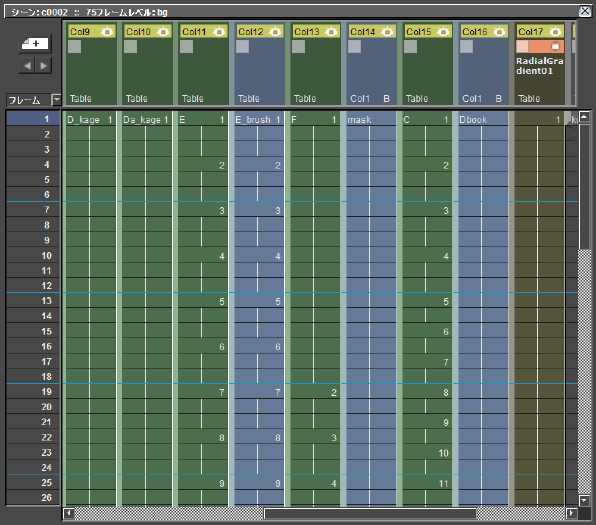
\includegraphics[width=13.8em]{OpenToonzInterfaceXsheet}}
\put(40,-148){\small Xsheet (Time Sheet)}
\put(190,-137){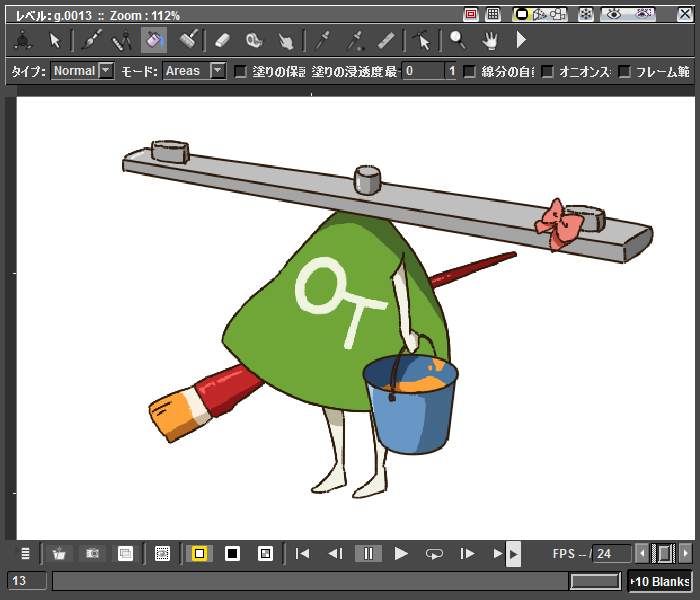
\includegraphics[width=14.15em]{OpenToonzInterfaceComboViewer}}
\put(210,-148){\small Combo Viewer (Main Viewer)}
\put(380,-119.5){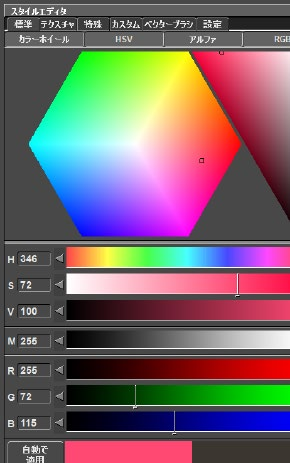
\includegraphics[width=6.7em]{OpenToonzInterfaceStyleEditor}}
\put(393,-128){\small Style Editor}
\put(380,-138){\small (ColorWheel,HSV,RGB)}
\put(4,-292){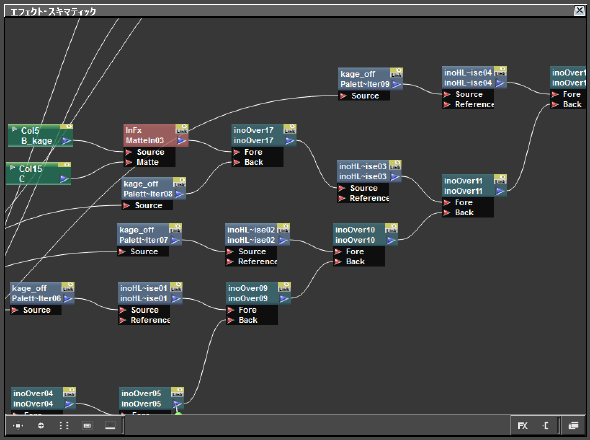
\includegraphics[width=13.8em]{OpenToonzInterfaceSchematic}}
\put(26,-303){\small Schematic (Nodes Editor)}
\put(184,-248){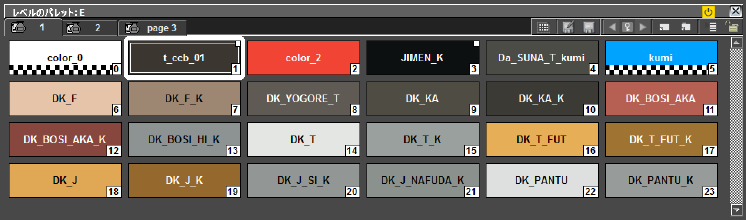
\includegraphics[width=17.2em]{OpenToonzInterfacePalette}}
\put(240,-259){\small Palette (Colors)}
\put(403.6,-335){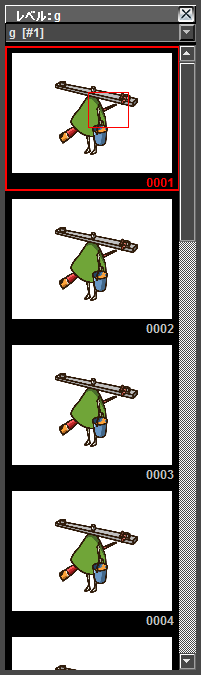
\includegraphics[width=4.7em]{OpenToonzInterfaceLevelStrip}}
\put(255,-290){\small Level Strip (Thumbnail View) →}
\end{picture}\\[25.9em]

\normalsize
\noindent ● Xsheet\\
Time Sheet interface (is called the Exposure Sheet = Xsheet in English). Place material into the\\
Scene, \& the timing of each material in the Video ID, you can determine a simple stacking order.\\
● Combo Viewer\\
It is used to preview all of the work you are doing by displaying the output picture.\\
● Style Editor\\
Used when editing the Color Palette. Color Wheel, HSV \& RGB values can be edited.\\
● Level Strip\\
A Thumbnail of each Cell Frame that is being edited are displayed in a row.\\
● Schematic\\
How Scene Effects are applied, tree structure of parent-child relationship geometric transforms.\\
● Palette\\
Displays the contents of the Palette file.\\
"Flipbook" panel is used for playing a sequence of images \& movies, \& "Color Model" panel is for\\
Color Picking on the Color Swatch Display when refining work, there are a variety of panels.\\
They can either be docked in each Room of the Main Window, or you can use them as a Floating\\
Window.

\newpage

\phantomsection
\section*{\uline{\hskip -3em \hskip 3em □ Column \& Level\hskip 12.5em}}
\addcontentsline{toc}{section}{□ Column \& Level}

\normalsize
\noindent Various materials (Cells, such as background material) can be arranged on the Xsheet (Time Sheet),\\
which are collectively known in OpenToonz as "Level". Level is stored in the Column on the Xsheet.\\
In each of the Cell (Frame) of the Column, no more than 1 Level / Video Number can be entered.\\
 As Column is a data structure unit of OpenToonz, it has an important meaning.\\
\large
① Column Level Container
\normalsize
\par
- 1 Cell in the Column can be, A) Empty, B) A non-sequence Level Frame\par
\ \ C) A Frame Level with a sequence numbered image. In the case of C),\par
\ \ the video sequence Frame Number is displayed on the Xsheet.\par
- Dealing with scenes in OpenToonz shooting, load material (Level) can\par
\ \ not be used to place over the Xsheet. The same applies to refining,\par
\ \ it doesn't matter as you don't want to display Xsheet panel, Level\par
\ \ read in LoadLevel is located in one of the Columns on the Xsheet.

\large
\noindent \begin{picture}(0,0)
\put(360,-35){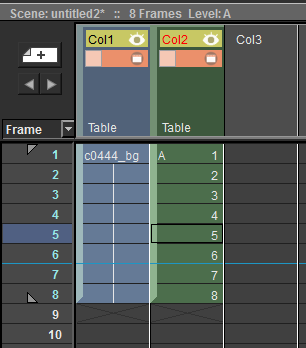
\includegraphics[width=12.1em]{ColumnLevelColumn}}
\end{picture}\\[-15em]

\noindent \hskip 34.2em 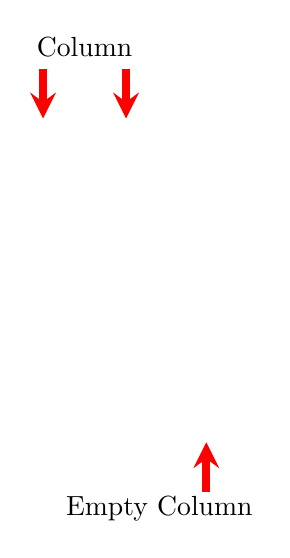
\begin{tikzpicture}
\draw[->,line width=3pt,red] (0em,-0.8em) to (0em,-2.6em);
\draw[->,line width=3pt,red] (3em,-0.8em) to (3em,-2.6em);
\draw[->,line width=3pt,red] (5.9em,-16.1em) to (5.9em,-14.3em);
\node at (1.5em,0em) {Column};
\node at (4.2em,-16.7em) {Empty Column};
\end{tikzpicture}\\[-6.3em]

\noindent ② Moving, Resizing Performed on the Column
\normalsize
\par
- Move, geometric transform data such as Resizing, Camera, Table, can\par
\ \  be given to Pegbar (Tap) or to each Column, we have a parent-child\par
\ \  relationship with the table as the parent. (Stage Schematic)\par
- The geometric conversion data for Level Images contained in each Column, will be deformed\\
\\[0.5em]
\large
③ Effects Synthesis Applied to the Column
\normalsize
\par
- Effects synthesis, will also be performed for each Column. Each Column Node contains the\par
\ \ Level material connected to the Effect Node, Effect processing is performed according to the\par
\ \ flow from the Left that leads into the Output Node on the Right. (Fx Schematic)\par
- Each of the Column Nodes, can output the image data of the Level contained within it

\large
\noindent \begin{picture}(0,0)
\put(0,-122){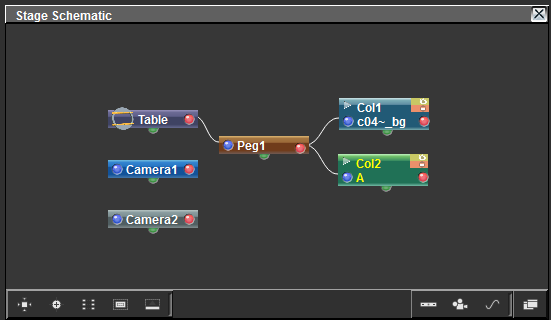
\includegraphics[width=17.8em]{ColumnLevelStageSchematic}}
\put(258,-122){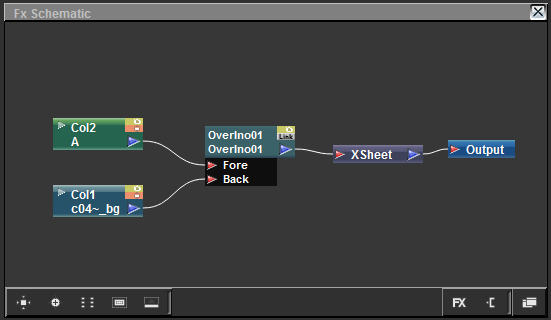
\includegraphics[width=17.8em]{ColumnLevelFxSchematic}}
\end{picture}\\[1.7em]

\noindent \hskip 14em 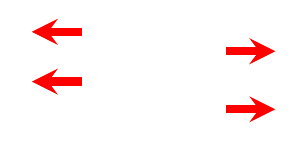
\begin{tikzpicture}
\draw[->,line width=3pt,red] (1.8em,0em) to (0em,0em);
\draw[->,line width=3pt,red] (1.8em,-1.8em) to (0em,-1.8em);
\draw[->,line width=3pt,red] (7em,-0.7em) to (8.8em,-0.7em);
\draw[->,line width=3pt,red] (7em,-2.8em) to (8.8em,-2.8em);
\end{tikzpicture}\\[1.9em]

\small
Stage Schematic (Left) \& FxSchematic (Right). Column Nodes (Red Arrows) (Empty Columns are not displayed)\\[3em]
\large
※ Xsheet Can Process Nested Structures
\normalsize
\par
\noindent As a special case, in 1 Level, you have the ability to summarize data of a plurality of Columns\\
as Xsheet of child (= SubXsheet). When selecting multiple Columns, the use of Collapse (Fold In\\
Sub-Sheet) command, you can put together the Column of selection to one Level of the SubXsheet.

\newpage

\phantomsection
\section*{\uline{\hskip -3em \hskip 3em □ Scene Editing Mode \& Level Editing Mode}}
\addcontentsline{toc}{section}{□ Scene Editing Mode \& Level Editing Mode}

\normalsize
\noindent OpenToonz animation software,  handles the time series (= Frame). OpenToonz has a mode where\\
you can select the 2 types of Frame, respectively, \& the Level of the Frame, called the Scene Frame.\\
\\
\large
○ Level Frame\\
\normalsize
When editing a single Level, the Frame will follow the Video Number you have in that Level.\\
When refining work, on a single one of each of the Video Number Levels, switch OpenToonz to the\\
\uline{Level Editing Mode}. When in Level Editing Mode, regardless of the arrangement on the Xsheet, the\\
main viewer displays only the picture of the selected current Frame of the Level (= Video Number).\\
\\
\uline{※ To Switch to the Level Editing Mode}\\
In LevelStrip navigate to where Thumbnails of the current Level are displayed, then left-click\\
on one of the Thumbnails.\\[0.5em]
\\
\large
○ Scene Frame\\
\normalsize
When you are editing a Scene, the Frame will follow the Row Number in Xsheet. Mainly when\\
shooting, while displaying a combination of all material that has been placed on the Xsheet,\\
Please Switch to the OpenToonz \uline{Scene Edit Mode}. When in Scene Editing Mode, CamStandVisibility\\
on Xsheet (Camera Stand Display) will be displayed on all of the Columns that are ON.\\
\\
※ Rendering Time \& CameraStandDisplay Column stacking uses the following order of priority\par
① Fx Schematic up \& down relationship between the Layer Synthesis Effects (Rendering Only)\par
② Z Depth Value\par
③ SO (Stacking Order) Value\par
④ Xsheet Order (Bottom Left, overlaps going to the Right)\\
\\
\uline{※ To Switch to the Scene Editing Mode}\\
Left-click on the left side of the Xsheet, Line Number \& the Area (= Scene Frame) is displayed.

\large
\noindent \begin{picture}(0,0)
\put(2,-163){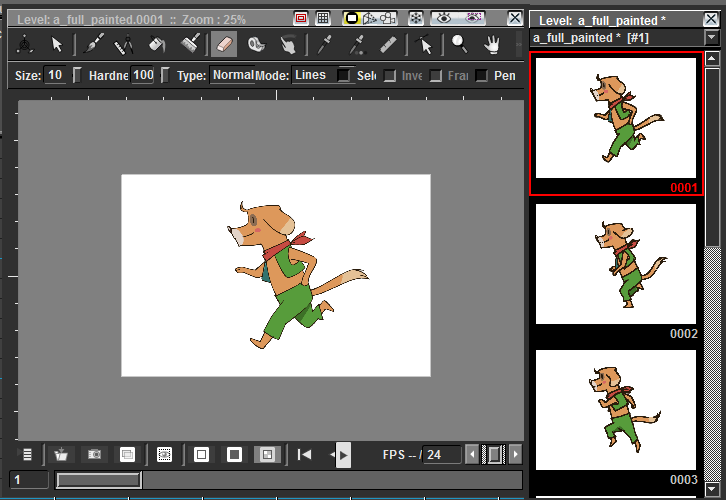
\includegraphics[width=18em]{EditModeLevel}}
\put(240,-163){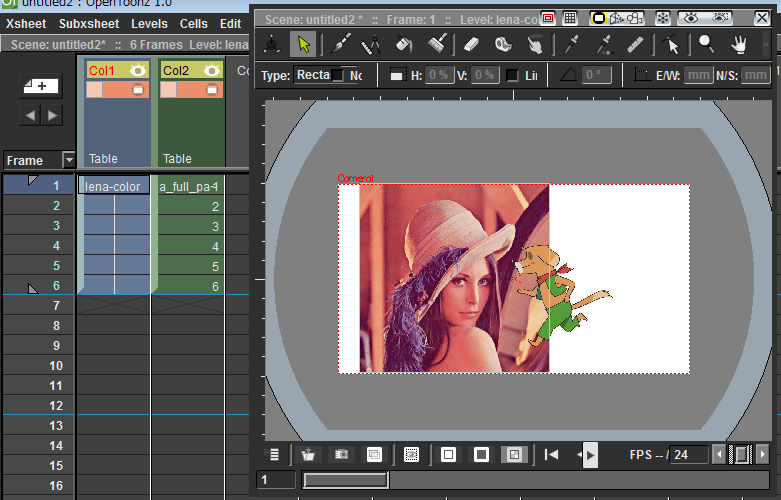
\includegraphics[width=19.35em]{EditModeScene}}
\end{picture}\\[10.5em]

\noindent \hskip 15.3em 
\begin{tikzpicture}
\draw[->,line width=3pt,red] (0em,-1.8em) to (0em,0em);
\draw[->,line width=3pt,red] (5.5em,-1.8em) to (5.5em,0em);
\end{tikzpicture}\\[-2.2em]

\small
\ Level Editing Mode (Left) \& Scene Editing Mode (Right). Left-click area to Switch Modes (Red Arrows).

\newpage

\newpage

\phantomsection
\section*{\uline{\hskip -3em \hskip 3em □ Room (Workspace)\hskip 11.5em}}
\addcontentsline{toc}{section}{□ Room (Workspace)}

\normalsize
\noindent In OpenToonz, trace, color designation, drawing \& refinement, photography, batch processing, are\\
inside a Room which combines panels to suit each type of data prepared in advance. You can switch\\
from the upper-right corner of the Room tab of the OpenToonz main window. When you switch the\\
Room, the contents of the menu bar is also switched to suit it. Each Rooms panel arrangement,\\
can be freely changed by the user, profile data is stored for each user, which loads on startup.

\large
\noindent \begin{picture}(0,0)
\put(4,-83){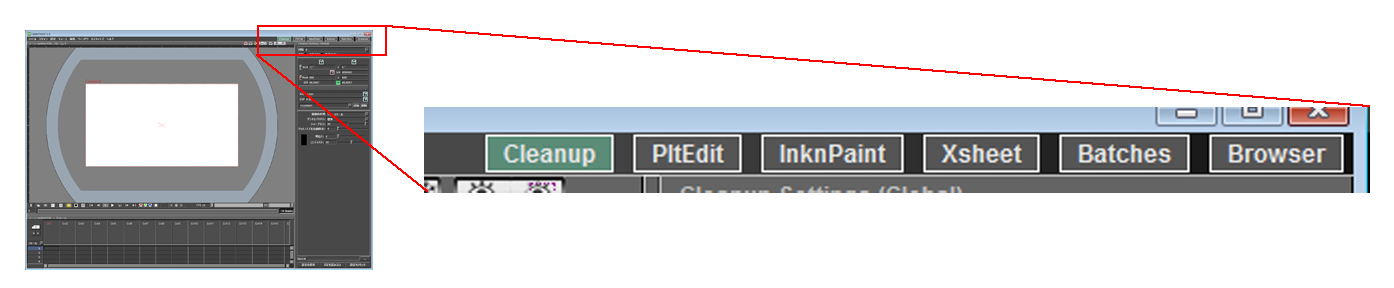
\includegraphics[width=39em]{RoomWorkSpaceTab}}
\put(285,-66){\normalsize Room Tab}
\end{picture}\\[6.4em]

\noindent ● To Start a Minimal Required Room \normalsize \colorbox{fontyellow}{\color{black}Intermediate Level}\\
If you want to work with shared users for each step of the animation, a good idea is to provide\\
a shortcut to start with the minimal Room necessary, to start-up faster.\\
Example: If you want to start with only a minimal open Room with "InknPaint" \& "Browser"\\
① [\$TOONZPROFILES]/layouts/OpenToonz.[User Name] You work in the [User Name] folder.\par
\ (By default, OpenToonz Stuff/profiles/layouts/OpenToonz.[User Name])\\
② Copy the layouts.txt, \& change it to an appropriate name. (Example: shiage\_layout.txt)\\
③ Open shiage\_layout.txt in e.g. WordPad, \& line up the Room config file names, as shown below,\\
leave only the corresponding Room lines ("InknPaint" is room3.ini, "Browser" is room6.ini),\\
deleting any other lines, \& save it.\\[-1em]
\par
\ \ \ \ \ \ \ \ room1.ini \ \ \ \ \ \ \ \ \ \ \ \ room3.ini\par
\ \ \ \ \ \ \ \ room2.ini \ \ \ \ \ \ \ \ \ \ \ \ room6.ini\par
\ \ \ \ \ \ \ \ room3.ini\par
\ \ \ \ \ \ \ \ room4.ini\par
\ \ \ \ \ \ \ \ room5.ini\par
\ \ \ \ \ \ \ \ room6.ini

\large
\noindent \begin{picture}(0,0)
\linethickness{0.1em}
\put(42,119){\line(1,0){67}}
\put(109,119){\line(0,-1){105}}
\put(109,14){\line(-1,0){67}}
\put(42,119){\line(0,-1){105}}
\put(153,119){\line(1,0){67}}
\put(221,119){\line(0,-1){105}}
\put(221,14){\line(-1,0){67}}
\put(153,119){\line(0,-1){105}}
\put(228,40){
\includegraphics[width=17em]{RoomWorkSpaceSpeechBubble}}
\put(251,61){\small Leave only the required Room file names}
\end{picture}\\[-8em]

\noindent \hskip 9.7em 
\begin{tikzpicture}
\draw[fill=arrowblue,arrowblue]  (1.6em,0em) --  (2.5em,-0.8em) --  (1.6em,-1.6em) -- (1.6em,-1.0em) -- (0em,-1.0em) -- (0em,-0.6em) -- (1.6em,-0.6em) -- cycle;
\end{tikzpicture}\\[2.5em]

\normalsize
\noindent ④ Create a shortcut to the OpenToonz executable file\\
⑤ Right-click the shortcut, \& open the properties\\
⑥ Add the end of the string, written in the "link",\par
\ \ -layout shiage\_layout.txt\par
\& then click OK.\\
⑦ When you start-up OpenToonz using this shortcut,\par
only the specified Room will be created.

\large
\noindent \begin{picture}(0,0)
\linethickness{0.1em}
\put(273,-57){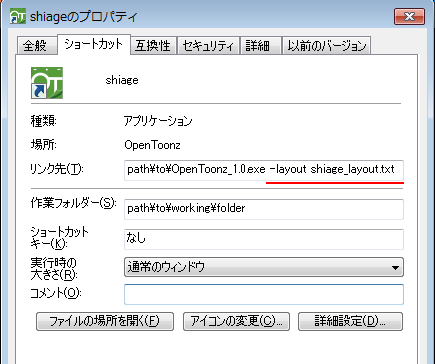
\includegraphics[width=18.7em]{RoomWorkSpaceShiageLayout}}
\put(11,-30){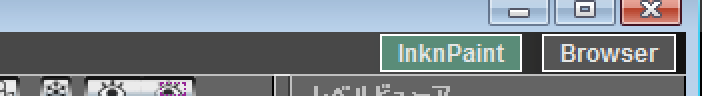
\includegraphics[width=20em]{RoomWorkSpaceInknPaintBrowser}}
\end{picture}

\newpage

\phantomsection
\section*{\uline{\hskip -3em \hskip 3em □ Project Data Management\hskip 8em}}
\addcontentsline{toc}{section}{□ Project Data Management}

\normalsize
\noindent In OpenToonz, the path \& default values of the Project Settings, such as Scene Settings, any work\\
which is newly created within the Project, is referred to as a "project", you can save into the\\
Working Folder of each Project (Project Folder) to store your material.\\
\\
\large
● sandbox Project\\
\normalsize
When starting OpenToonz for the first time, the Current Project is called\\
sandbox, it is the default Project. Looking at the FileBrowser panel on\\
the Folder Tree, the Circle Node on the Left side of "sandbox" is turned\\
Red. This is a sign that the Current sandbox Project has been Selected.

\large
\noindent \begin{picture}(0,0)
\linethickness{0.1em}
\put(365,-35){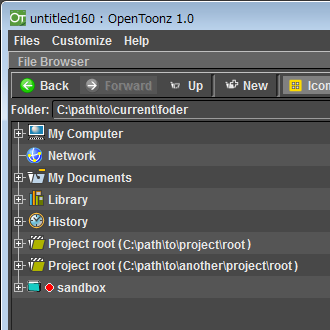
\includegraphics[width=13.2em]{ProjectDataManagementSandboxProject}}
\end{picture}\\

\noindent ● To Create a Project\\
\normalsize
① Browse using the Menu Bar in the Workspace, select File > New Project, \& in the following\\
input boxes, specify the path to each of the Project Folders.\\
\par
\hskip 21em ← To select storage location of the Project Settings\\
\par
\hskip 21em ← Project Name\\[-1em]
\par
\small
\hskip 26em Enter the path to each of the Project Folders.\par
\hskip 26em Assumed to store the files in the following manner.\par
\hskip 26em +inputs: Scanned Images (Such as TIFF)\par
\hskip 26em +drawings: Toonz Level Material (TLV + PLT \& PLI)\par
\hskip 26em +scenes: Scene File (TNZ)\par
\hskip 26em +extras: Background Image Files, Audio Files, etc.\par
\hskip 26em +outputs: Rendered Image Output\par
\hskip 26em +palettes: Color Swatch (PLT). Studio Palette Panel\par
\hskip 26em also referred to as the Project Palette.\par
\hskip 26em +scripts: Script Files

\large
\noindent \begin{picture}(0,0)
\linethickness{0.1em}
\put(-2,20){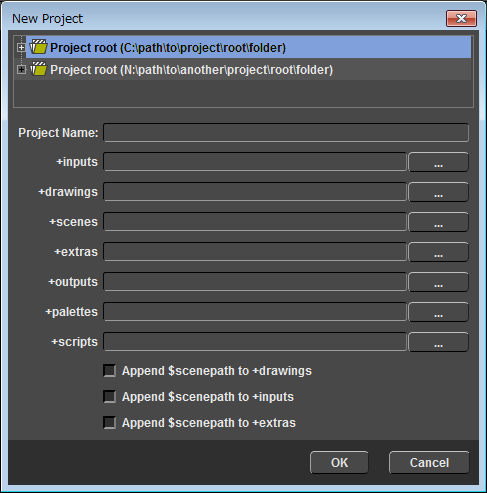
\includegraphics[width=18.2em]{ProjectDataManagementCreateProject}}
\linethickness{0.1em}
\put(223,170){\line(1,0){9}}
\put(232,161){\line(1,0){9}}
\put(232,170){\line(0,-1){92}}
\put(223,78){\line(1,0){9}}
\end{picture}\\[-2.5em]

\normalsize
\noindent ※ The path string in \$scenepath is the current scene name, it is assigned when a file is saved.\\
\\
② Press OK, \& the project is created, it becomes the current project.\\
A new Project Node is added To FileBrowser panel on the Left side of the\\
Folder Tree, \& you will see that the Red marker has moved accordingly.\\
\\
\large
● To Switch the Project\\
\normalsize
When you click the Circle Node to the Left of a Project Name, the Circle\\
will be marked Red, \& will switch the current project.

\large
\noindent \begin{picture}(0,0)
\linethickness{0.1em}
\put(365,-25){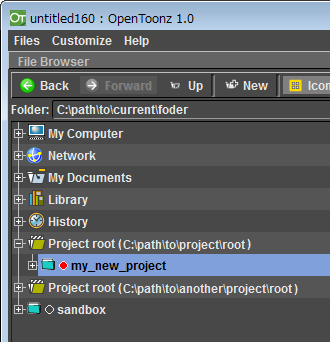
\includegraphics[width=13.2em]{ProjectDataManagementSwitchProject}}
\end{picture}\\

\newpage

\noindent● To Change the Project Folder\\
\normalsize
In the Browser Room, run Files > Project Settings... Edit the Project Folder path, \& close the\\
dialog.\\
\large
● To Set the Current Scene to the Specified Values of the Project\\
\normalsize
In the Browser Room, run Files > Save Default Settings.\\
\\[0.5em]
\large
● To Work Without Creating a Project\\
\normalsize
Project based Data Management, can shorten the workload, such as with the stored material inside\\
the file path "+drawings", it is possible to simplify the data management, also there is a big\\
advantage to having default project values set for a common scene.\\
On the other hand, in case of use such as when performing finished outsourced work, such as\\
dealing with small amounts of data from a variety of scenes, the advantage of summarized data for\\
each piece is small, it would be inconvenient to create a project for each one. In such a case,\\
without creating a project, please work by using the Default Project "sandbox". The User Project\\
Folder of the project that was created \& any Scene Files stored outside of the sub-folders, are\\
recognized as belonging to the sandbox Project, the user can also proceed without using a project.\\

\end{document}